% Options for packages loaded elsewhere
\PassOptionsToPackage{unicode}{hyperref}
\PassOptionsToPackage{hyphens}{url}
\PassOptionsToPackage{dvipsnames,svgnames*,x11names*}{xcolor}
%
\documentclass[
]{article}
\usepackage{lmodern}
\usepackage{amssymb,amsmath}
\usepackage{ifxetex,ifluatex}
\ifnum 0\ifxetex 1\fi\ifluatex 1\fi=0 % if pdftex
  \usepackage[T1]{fontenc}
  \usepackage[utf8]{inputenc}
  \usepackage{textcomp} % provide euro and other symbols
\else % if luatex or xetex
  \usepackage{unicode-math}
  \defaultfontfeatures{Scale=MatchLowercase}
  \defaultfontfeatures[\rmfamily]{Ligatures=TeX,Scale=1}
  \setmainfont[]{Linux Libertine O}
\fi
% Use upquote if available, for straight quotes in verbatim environments
\IfFileExists{upquote.sty}{\usepackage{upquote}}{}
\IfFileExists{microtype.sty}{% use microtype if available
  \usepackage[]{microtype}
  \UseMicrotypeSet[protrusion]{basicmath} % disable protrusion for tt fonts
}{}
\makeatletter
\@ifundefined{KOMAClassName}{% if non-KOMA class
  \IfFileExists{parskip.sty}{%
    \usepackage{parskip}
  }{% else
    \setlength{\parindent}{0pt}
    \setlength{\parskip}{6pt plus 2pt minus 1pt}}
}{% if KOMA class
  \KOMAoptions{parskip=half}}
\makeatother
\usepackage{xcolor}
\IfFileExists{xurl.sty}{\usepackage{xurl}}{} % add URL line breaks if available
\IfFileExists{bookmark.sty}{\usepackage{bookmark}}{\usepackage{hyperref}}
\hypersetup{
  pdftitle={Algorithmic Pattern},
  pdfauthor={Alex McLean},
  colorlinks=true,
  linkcolor=Maroon,
  filecolor=Maroon,
  citecolor=Blue,
  urlcolor=Blue,
  pdfcreator={LaTeX via pandoc}}
\urlstyle{same} % disable monospaced font for URLs
\usepackage{color}
\usepackage{fancyvrb}
\newcommand{\VerbBar}{|}
\newcommand{\VERB}{\Verb[commandchars=\\\{\}]}
\DefineVerbatimEnvironment{Highlighting}{Verbatim}{commandchars=\\\{\}}
% Add ',fontsize=\small' for more characters per line
\usepackage{framed}
\definecolor{shadecolor}{RGB}{240,240,240}
\newenvironment{Shaded}{\begin{snugshade}}{\end{snugshade}}
\newcommand{\AlertTok}[1]{\textcolor[rgb]{0.94,0.16,0.16}{#1}}
\newcommand{\AnnotationTok}[1]{\textcolor[rgb]{0.56,0.35,0.01}{\textbf{\textit{#1}}}}
\newcommand{\AttributeTok}[1]{\textcolor[rgb]{0.77,0.63,0.00}{#1}}
\newcommand{\BaseNTok}[1]{\textcolor[rgb]{0.00,0.00,0.81}{#1}}
\newcommand{\BuiltInTok}[1]{#1}
\newcommand{\CharTok}[1]{\textcolor[rgb]{0.31,0.60,0.02}{#1}}
\newcommand{\CommentTok}[1]{\textcolor[rgb]{0.56,0.35,0.01}{\textit{#1}}}
\newcommand{\CommentVarTok}[1]{\textcolor[rgb]{0.56,0.35,0.01}{\textbf{\textit{#1}}}}
\newcommand{\ConstantTok}[1]{\textcolor[rgb]{0.00,0.00,0.00}{#1}}
\newcommand{\ControlFlowTok}[1]{\textcolor[rgb]{0.13,0.29,0.53}{\textbf{#1}}}
\newcommand{\DataTypeTok}[1]{\textcolor[rgb]{0.13,0.29,0.53}{#1}}
\newcommand{\DecValTok}[1]{\textcolor[rgb]{0.00,0.00,0.81}{#1}}
\newcommand{\DocumentationTok}[1]{\textcolor[rgb]{0.56,0.35,0.01}{\textbf{\textit{#1}}}}
\newcommand{\ErrorTok}[1]{\textcolor[rgb]{0.64,0.00,0.00}{\textbf{#1}}}
\newcommand{\ExtensionTok}[1]{#1}
\newcommand{\FloatTok}[1]{\textcolor[rgb]{0.00,0.00,0.81}{#1}}
\newcommand{\FunctionTok}[1]{\textcolor[rgb]{0.00,0.00,0.00}{#1}}
\newcommand{\ImportTok}[1]{#1}
\newcommand{\InformationTok}[1]{\textcolor[rgb]{0.56,0.35,0.01}{\textbf{\textit{#1}}}}
\newcommand{\KeywordTok}[1]{\textcolor[rgb]{0.13,0.29,0.53}{\textbf{#1}}}
\newcommand{\NormalTok}[1]{#1}
\newcommand{\OperatorTok}[1]{\textcolor[rgb]{0.81,0.36,0.00}{\textbf{#1}}}
\newcommand{\OtherTok}[1]{\textcolor[rgb]{0.56,0.35,0.01}{#1}}
\newcommand{\PreprocessorTok}[1]{\textcolor[rgb]{0.56,0.35,0.01}{\textit{#1}}}
\newcommand{\RegionMarkerTok}[1]{#1}
\newcommand{\SpecialCharTok}[1]{\textcolor[rgb]{0.00,0.00,0.00}{#1}}
\newcommand{\SpecialStringTok}[1]{\textcolor[rgb]{0.31,0.60,0.02}{#1}}
\newcommand{\StringTok}[1]{\textcolor[rgb]{0.31,0.60,0.02}{#1}}
\newcommand{\VariableTok}[1]{\textcolor[rgb]{0.00,0.00,0.00}{#1}}
\newcommand{\VerbatimStringTok}[1]{\textcolor[rgb]{0.31,0.60,0.02}{#1}}
\newcommand{\WarningTok}[1]{\textcolor[rgb]{0.56,0.35,0.01}{\textbf{\textit{#1}}}}
\usepackage{graphicx}
\makeatletter
\def\maxwidth{\ifdim\Gin@nat@width>\linewidth\linewidth\else\Gin@nat@width\fi}
\def\maxheight{\ifdim\Gin@nat@height>\textheight\textheight\else\Gin@nat@height\fi}
\makeatother
% Scale images if necessary, so that they will not overflow the page
% margins by default, and it is still possible to overwrite the defaults
% using explicit options in \includegraphics[width, height, ...]{}
\setkeys{Gin}{width=\maxwidth,height=\maxheight,keepaspectratio}
% Set default figure placement to htbp
\makeatletter
\def\fps@figure{htbp}
\makeatother
\setlength{\emergencystretch}{3em} % prevent overfull lines
\providecommand{\tightlist}{%
  \setlength{\itemsep}{0pt}\setlength{\parskip}{0pt}}
\setcounter{secnumdepth}{5}
\newlength{\cslhangindent}
\setlength{\cslhangindent}{1.5em}
\newenvironment{cslreferences}%
  {\setlength{\parindent}{0pt}%
  \everypar{\setlength{\hangindent}{\cslhangindent}}\ignorespaces}%
  {\par}

\title{Algorithmic Pattern}
\author{Alex McLean}
\date{}

\begin{document}
\maketitle

\hypertarget{defining-algorithmic-pattern}{%
\subsection{Defining algorithmic
pattern}\label{defining-algorithmic-pattern}}

This paper explores the world of algorithmic pattern, and the ways in
which it offers an interface to the computer musician. Let's first look
at the words pattern and algorithm separately, before putting them
together.

Patterns are present everywhere, certainly in textiles, choreography,
mathematics, design and music. However, at first glance, the use of the
word in music seems comparatively impoverished, at least in the West. At
the time of writing, the English language wikipedia page on pattern has
no mention of music, and furthermore, when musicians refer to a pattern,
they usually mean any sequence that repeats. The word can even take on a
pejorative sense in music, for example in a conference paper on
transdisciplinary collaboration Hugill recounts how (and I paraphrase)
mathematicians spend their careers searching for patterns, while many
composers will be seriously offended if you accuse them of making
patterns.

By comparison, pattern in textiles is alive with compositional
techniques, not only repetitions but reflections and symmetries, and
generative structural compositions. Once you scratch the surface
however, music is of course also alive with patterns across
compositional techniques. For example, the familiar canon structures,
where one voice imitates another, played over the top with a delay. So
it seems that the difference here is the way words are used; in music, a
canon contains patterns, whereas in textiles, such a structure based on
glide symmetry could itself be referred to as the pattern.

What \emph{is} a Pattern? Grünbaum and Shephard define patterns as
``designs repeating some motif in a more or less systematic manner.''
They write in the context of geometric tilings, but the same definition
largely holds in the music fields; a sequence becomes a pattern, once it
is repeated. However, in music we too often focus on the repetition, and
not the systematic manner in which it is repeated. For a pattern to be
interesting, we need to do more than repeat it; the repetition only
provides the metrical ground on which the pattern acts. Looking around
the room you are in now, you will likely see patterns of repetition, but
also of reflection, rotation, interference/moire, and glitch. The
textiles around (or on) you may well have a visual pattern arising not
from the colour of threads alone, but from computational interference
between colour and structure.

Accordingly, in the present paper, we focus on pattern as a whole family
of techniques for working with regularites in the world. Such patterns
allow us to perceive repetition, reflection and interference in a
material. In other words, the way we percieve pattern is inextricably
linked with the structured movements of its making. And, once we are
dealing with `structure movements of making', we are in the world of
algorithms.

An \emph{algorithm} is a step-by-step set of instructions. Sometimes it
is assumed that by a step-by-step set, we mean a sequence of
instructions, but this is not the case; indeed the notion of an
algorithm has been formalised as lambda calculus, which may involve
recursive steps in to a function declaration, rather than stepping down
a stateful sequence of instructions. This clarification becomes
important later in this paper, when we address TidalCycles, a live
coding environment embedded in the Haskell language, which is itself
based on lambda calculus.

So, there is some sense that the words algorithm and pattern are
synonyms, and therefore the phrase ``algorithmic pattern'' is a
tautology. This phrase is nonetheless useful for on one hand for
clarifying that we address algorithms not just as software engineering
tools, but as formalised ways of making that can be perceived in
end-results. On the other hand, it clarifies that patterns are not
simple sequences, but structural qualities. This builds a perspective
that creates a generative and perceptual connection between creation and
reception.

\hypertarget{patterns-in-nime}{%
\subsection{Patterns in NIME}\label{patterns-in-nime}}

The meaning of \emph{algorithmic pattern} has a particular resonance in
interface design, especially in the NIME (New Interfaces for Musical
Expression) field. When we write something as an algorithmic pattern, we
work at least one step removed from the surface of a `target domain'
such as musical notes. By analogy, we don't hit the drum, we write about
hitting the drum. Not even that, we write about relationships between
drum hits, the structures that lead to one movement following another.
This is a trade off, which creates distance between ourselves and an
instrument, losing direct tactile control, but which brings us `up' to
work on a compositional, structural level. Here, we lose physical
connection to a drum skin, but instead work in a way where a very small
change can create far reaching, even unexpected changes in the music as
it unfolds. This generative relationship with algorithmic pattern is
what we explore in the following, taking first live coding of music, and
then live weaving of textiles as comparative examples.

As things stand, what does the word pattern mean to NIME authors?
According to use of the \texttt{pdfgrep} utility on a corpus of 1,739
NIME papers, word `pattern' can be found in 803 papers (46\% of the
total) of which 315 (18\% of the total) contain it more than twice.
These were ranked by incidence of the word, and the top twenty sampled
and examined (ranging from 26 to 150 occurrences per paper), to gain an
impression of how the word is used in the community. Of these twenty
papers, I deemed only one (Faubel 2014) explored pattern as an activity,
in the context of patterns of interaction emerging and continually
changing in motor feedback loops. Of the remaining papers, nine
discussed transformation of patterns in some way (Eigenfeldt and Kapur
2008, @Ogawa2009, @Jordnicode2252016, @Lee:2012a, @Kitani2010,
@Toka2018, @Hawryshkewich2010, @rvogl2017), although referred to
patterns as the end result, rather than as a generation or
transformation process or notation. The remaining eleven papers
(Schoonderwaldt and Jensenius 2011, @Derbinsky2012, @slui2014, @Lee2006,
@Trail:2012a, @Bouillot2007, @Kim2013, @Lee2007, @Petit2019,
@Rauber--Du--Bois2019, Subramanian2012@) referred to patterns as fixed
sequences. There are no satisfying definitions of pattern, although
Petit and serrano (2019) writes ``A pattern can be any part of a score,
a MIDI sequence, or a pre-recorded sound''.

Wanting to find more examples of papers treating pattern as activity or
behaviour rather than sequence, I searched again with the gerund
patterning. This returned nine papers, none of which had more than two
instances of the word. Most were passing references, but Green (2014)
used patterning to refer to the combination of two patterns, Suiter
(2010) described musical form as a process, and patterns in terms of how
they relate to one another, Collins and McLean (2014) as live coded
algorithms as patterned behaviour, and Gimenes, Miranda, and Johnson
(2007) quote Meyer in defining a composer's style as connecting patterns
in human behaviour with patterns in results. I count all of these as
fitting the definition of algorithmic pattern.

\hypertarget{algorithmic-pattern-in-computer-music-interfaces}{%
\subsection{Algorithmic Pattern in Computer Music
Interfaces}\label{algorithmic-pattern-in-computer-music-interfaces}}

Algorithmic and generative music systems often come with high-minded
claims of infinite variation or artificial intelligence. However on
closer examination, these systems often rely upon surprisingly simple
systems based on probability (e.g.~`Markov chains'), arbitrary decisions
(randomness/chance) and straightforward sequencing, called `algorithmic'
simply because they are expressed as text rather than as a graphical
piano roll. In her foundational essay ``Manipulations of Musical
Patterns'', Spiegel (1981) looks beyond such methods, arguing
convincingly for greater focus on pattern transformations in computer
music interfaces, naming twelve categories of pattern transformation
which, Spiegel argues, should be as central to computer music interfaces
as copy and paste.

Our argument is not however that algorithmic pattern is complex.
Musician and sound artist Mark Fell is one example of someone who fully
embraces simplicity of a pattern-based approach to sound. In ``Notes on
Pattern Synthesis'', ({\textbf{???}}) introduces the Max patches behind
his acclaimed album Multistability, which work as studies of interaction
within self-enforced guidelines. This minimalist approach results in
music has great clarity, but is nonetheless complex in structure. The
usual minimalist examples, such as Reich's clapping music fit here too.
Simple in its patterned construction, but bringing forth astonishing
detail in its outcome. This is core benefit to using a pattern as an
interface, embracing the simplest ingredients, but transforming them and
composing them together to create complex results. Far from new, this
approach grounds discussion of music generation in a rich perspective,
able to draw from an expansive variety of cultural practices and
artefacts from around the world and across history. Pattern is a
universal.

In the following paper, we explore the expansive world of pattern
in-depth. One perspective will be from computer music, with focus on the
representation and manipulation of pattern in the TidalCycles
environment. However, pattern is a universal concept, and we will also
look at examples from textiles, particularly interference patterns in
weaves and braids.

\hypertarget{pattern-in-tidalcycles}{%
\subsection{Pattern in TidalCycles}\label{pattern-in-tidalcycles}}

Work on TidalCycles (commonly \emph{Tidal} for short) first began in
2009, and over the past decade has developed into a comprehensive,
free/open source environment for algorithmic pattern, mainly in the
context of live coding music. At heart, it is a domain specific language
(DSL) and environment for patterning Open Sound Control network messages
({\textbf{???}}), embedded in the pure functional language Haskell.
Tidal is most commonly used in tandem with the SuperDirt software, a
hybrid framework for sample manipulation, synthesis and MIDI,
implemented in SuperCollider. However, Tidal can be applied to any kind
of pattern, and has indeed been used to pattern live choreographic
scores ({\textbf{???}}), woven textiles ({\textbf{???}}), DMX-controlled
lighting, and VJing.

While Tidal has been developed alongside creative practice, it upholds
strong computer scientific principles. Crucially, a pattern is defined
as a pure function, and therefore may be composed with other patterns
flexibly and safely. As Tidal has developed, its core representation has
grown more succinct, and a recent rewrite resulted in more rigorous
understanding of what, in terms of Tidal, a pattern \emph{is}. Tidal
types Much, but not all of Tidal's notion of pattern comes from the way
it represents pattern within Haskell's type system, as a pure function
of time. This folllows work on pure functional reactive programming,
where rather than representing data using lists, behaviour is
represented, with functions. Accordingly, rather than representing a
sequence as a list of events, Tidal represents it as a function, which
takes a timespan as input, and returns all the events which are active
during that time. In this way, the idea of a pattern being about
behaviour rather than a sequence is embedded in Tidal's core.

Lets have a look at the type declarations themselves, describing each
for those unfamiliar with the Haskell language.

\begin{Shaded}
\begin{Highlighting}[]
\KeywordTok{data} \DataTypeTok{Arc} \OtherTok{=} \DataTypeTok{Arc}\NormalTok{ \{}\OtherTok{start ::} \DataTypeTok{Rational}\NormalTok{,}\OtherTok{ stop ::} \DataTypeTok{Rational}\NormalTok{\}}
\end{Highlighting}
\end{Shaded}

A timespan is expressed as an arc of time, consisting of a start and end
time. Timespans are referred to as arcs, in sympathy with a cyclic
notion of time. Importantly, time is represented at a rational (rather
than floating point or integral) number, therefore allowing time to be
arbitrarily subdivided with 100\% accuracy.

\begin{Shaded}
\begin{Highlighting}[]
\KeywordTok{data} \DataTypeTok{Event}\NormalTok{ a }\OtherTok{=} \DataTypeTok{Event}\NormalTok{ \{}
\OtherTok{    whole ::} \DataTypeTok{Maybe} \DataTypeTok{Arc}\NormalTok{,}
\OtherTok{    part ::} \DataTypeTok{Arc}\NormalTok{,}
\OtherTok{    value ::}\NormalTok{ a}
\NormalTok{\}}
\end{Highlighting}
\end{Shaded}

An event contains a value of some type \texttt{a}, and two arcs. The
\texttt{part} arc represents the timespan during which the event is
active. An event may be a fraction of an event, in which case the
`whole' arc gives the timespan for the original. If a whole is not set,
this indicates that the event is analogue; that is, rather than having a
discrete beginning and end, the value continuously changes, and the one
that is returned is sampled at the midpoint of the query arc. This
approach allows both discrete and continuously varying events to
co-exist in the same pattern.

\begin{Shaded}
\begin{Highlighting}[]
\KeywordTok{type} \DataTypeTok{Query}\NormalTok{ a }\OtherTok{=}\NormalTok{ (}\DataTypeTok{Arc} \OtherTok{{-}>}\NormalTok{ [}\DataTypeTok{Event}\NormalTok{ a])}
\KeywordTok{data} \DataTypeTok{Pattern}\NormalTok{ a }\OtherTok{=} \DataTypeTok{Pattern}\NormalTok{ \{}\OtherTok{query ::} \DataTypeTok{Query}\NormalTok{ a,}
\OtherTok{                          controls ::} \DataTypeTok{StateMap}
\NormalTok{\}}
\end{Highlighting}
\end{Shaded}

A query represents the pattern's behaviour, as a function from time to
events. In particular, a query takes an arc as input, and returns a set
of events which are active during that arc as output. The values of the
events must all be of the same type, and the parts of the events will be
contrained to the query arc. If an event's `whole' extends beyond the
query, it is returned as-is, but its `part' is curtailed. In other
words, you may be returned a fragment of an event for a given query, but
will still have access to the arc of the whole, of which the event is
part.

\hypertarget{tidal-composition}{%
\subsubsection{Tidal composition}\label{tidal-composition}}

The above strict definition of pattern does not say much about Tidal as
an interface, but what follows from it is a rich approach to
composition, supported by a large library of pattern combinators.
Composition is meant here in both a musical and computer scientific
sense, in terms of composing together musical behaviours into new,
generally more complex behaviours. Tidal supports a multitude of ways to
combine patterns together, most ride on how Tidal allows you to simply
treat patterns as values, allowing you to take any function that
combines two values, and use it to combine two patterns of values.

As a trivial example, lets combine two tidal patterns
\texttt{fastcat\ {[}1,2,3{]}} and \texttt{fastcat\ {[}4,5{]}}. The first
thing to note is that \texttt{fastcat} combines a list of patterns by
concatenating them in a contiguous sequence, of equal durations over a
cycle. The notion of a metrical cycle is important here, as it is most
often the reference point in a composition, rather than a beat or step.
So, we are combining two patterns with different structures - one has
three events per cycle, and the other has two. We can visualise them
like this:

\begin{Shaded}
\begin{Highlighting}[]
\NormalTok{fastcat [}\DecValTok{1}\NormalTok{,}\DecValTok{2}\NormalTok{,}\DecValTok{3}\NormalTok{]}
\end{Highlighting}
\end{Shaded}


\includegraphics[width=1\textwidth,height=\textheight]{figures/2efc8e658200e8b94a2bd3f87ef273ce_0.pdf}

\begin{Shaded}
\begin{Highlighting}[]
\NormalTok{fastcat [}\DecValTok{4}\NormalTok{,}\DecValTok{5}\NormalTok{]}
\end{Highlighting}
\end{Shaded}


\includegraphics[width=1\textwidth,height=\textheight]{figures/a5de1a12bad00c7c2d103e9b5e3f75f5_0.pdf}

The default way to combine them is with \texttt{+}, producing the
following:

\begin{Shaded}
\begin{Highlighting}[]
\NormalTok{fastcat [}\DecValTok{1}\NormalTok{,}\DecValTok{2}\NormalTok{,}\DecValTok{3}\NormalTok{] }\OperatorTok{+}\NormalTok{ fastcat [}\DecValTok{4}\NormalTok{,}\DecValTok{5}\NormalTok{]}
\end{Highlighting}
\end{Shaded}


\includegraphics[width=1\textwidth,height=\textheight]{figures/5a95fc0670ae3bb993fa97b33c8937f8_0.pdf}

You can see that in the above, \texttt{1} gets added to part of
\texttt{4}, \texttt{2} gets split between \texttt{4} and \texttt{5}, and
\texttt{3} gets added to part of \texttt{5}. An alternative operator,
\texttt{\textbar{}+}, privileges structure on the left. The same events
are matched up, but the resulting events maintain the `wholes' from the
pattern on the left hand side of the operator:

\begin{Shaded}
\begin{Highlighting}[]
\NormalTok{fastcat [}\DecValTok{1}\NormalTok{,}\DecValTok{2}\NormalTok{,}\DecValTok{3}\NormalTok{] }\OperatorTok{|+}\NormalTok{ fastcat [}\DecValTok{4}\NormalTok{,}\DecValTok{5}\NormalTok{]}
\end{Highlighting}
\end{Shaded}

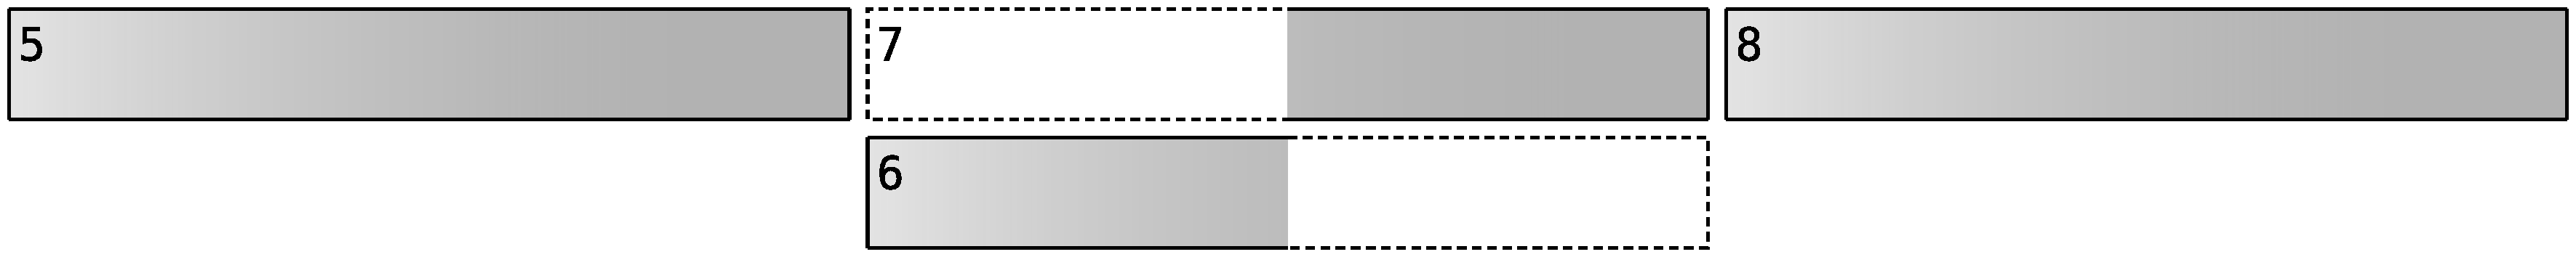
\includegraphics[width=1\textwidth,height=\textheight]{figures/df0a301c3ac358e46fab2b793f180e9f_0.pdf}

Conversely, the \texttt{+\textbar{}} operator privileges structure from
the right hand pattern:

\begin{Shaded}
\begin{Highlighting}[]
\NormalTok{fastcat [}\DecValTok{1}\NormalTok{,}\DecValTok{2}\NormalTok{,}\DecValTok{3}\NormalTok{] }\OperatorTok{+|}\NormalTok{ fastcat [}\DecValTok{4}\NormalTok{,}\DecValTok{5}\NormalTok{]}
\end{Highlighting}
\end{Shaded}

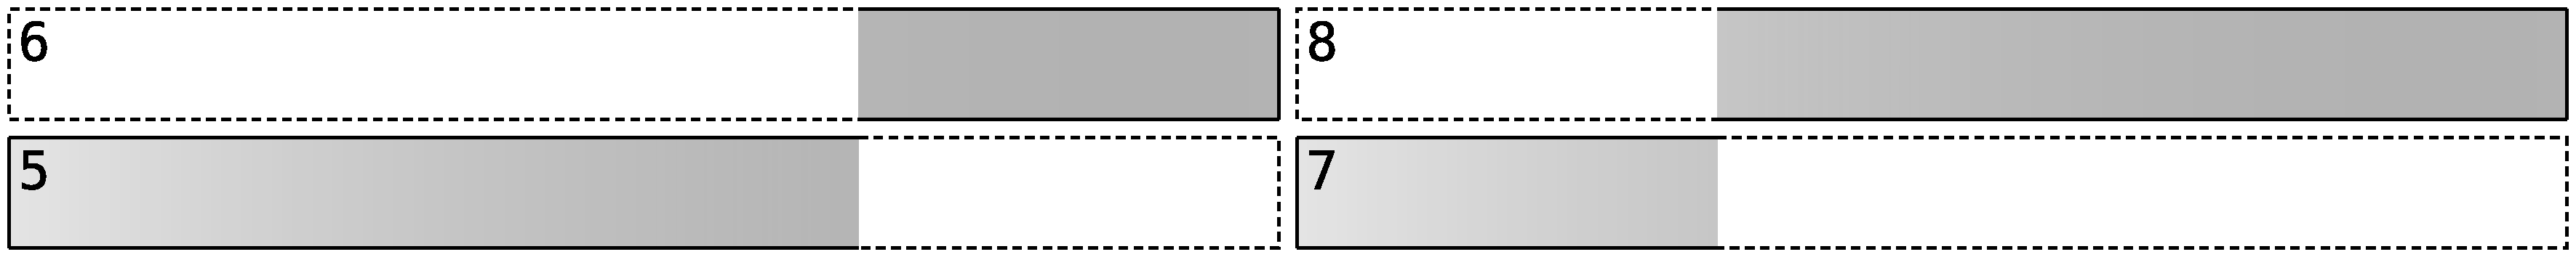
\includegraphics[width=1\textwidth,height=\textheight]{figures/97e25ab63906058b5e790f194888828d_0.pdf}

Note that when such a pattern structure reaches the scheduler, only the
events that have their onsets intact will result in an event actually
being triggered. That is, the start of an event's `part' must be the
same as an event's `whole' to result in sound, otherwise it represents a
fragment of an event's tail, only useful for combining with other
events. However, a model that works beyond trigger messages, allowing
continual varying of a sound's parameters after it has been triggered,
is at working prototype stage.

There is a library of such operators for basic arithmetic, but any
function can be used to combine patterns together in this way by using
Haskell's standard syntax for applicative functors, with Tidal's
additional nonstandard operators \texttt{\textless{}*} and
\texttt{*\textgreater{}} for privileging structure on the left or right.
For example, to merge two colour patterns:

\begin{Shaded}
\begin{Highlighting}[]
\NormalTok{blend }\OperatorTok{<$>}\NormalTok{ (slow }\DecValTok{4}\NormalTok{ sine) }\OperatorTok{*>} \StringTok{"red"} \OperatorTok{<*>} \StringTok{"blue orange"}
\end{Highlighting}
\end{Shaded}


\includegraphics[width=5in,height=\textheight]{figures/bd8761a5cc87209b083bb9fdc4fe12b9_gradient_0.pdf}

Instead of using `fastcat', the above

It is worth reiterating at this point that patterns are functions, and
not data structures. By combining them in this way we are not computing
anything, only creating a new pattern function composed of other pattern
functions. No calculation actually take place until the resulting
pattern is queried.

\hypertarget{patterned-parameters}{%
\subsubsection{Patterned parameters}\label{patterned-parameters}}

TidalCycles has a large library of combinators, but for the purpose of
this paper we will focus on just one, the \texttt{fast} function, which
simply speeds up (or for factors \textless{} 1 slows down) a pattern.
Its definition is minimal, taking a time factor and a target pattern as
input, and manipulating the target pattern's timeline according to the
factor:

\begin{Shaded}
\begin{Highlighting}[]
\NormalTok{fast timepat pat }\OtherTok{=}
\NormalTok{  innerJoin ((\textbackslash{}time }\OtherTok{{-}>}\NormalTok{ withResultTime (}\OperatorTok{/}\NormalTok{ time) }\OperatorTok{$}
\NormalTok{                         withQueryTime (}\OperatorTok{*}\NormalTok{ time) pat)}
              \OperatorTok{<$>}\NormalTok{ timepat}
\NormalTok{            )}
\end{Highlighting}
\end{Shaded}

What is interesting in the above is that \emph{the time factor input is
itself a pattern}. With combined used of the
\texttt{\textless{}\$\textgreater{}} operator and \texttt{innerJoin}
function, we manipulate the target pattern \emph{inside} the pattern of
time. This higher order magic uses the much same procedure for combining
patterns described above. The result is a highly flexible function for
patterning the speed of a pattern. For example:

\begin{Shaded}
\begin{Highlighting}[]
\NormalTok{fast }\DecValTok{4} \OperatorTok{$}\NormalTok{ fast }\StringTok{"1 2 3"} \StringTok{"white pink red orange"}
\end{Highlighting}
\end{Shaded}

\includegraphics[width=5in,height=\textheight]{figures/43220a67b5b9a766c3b9b0b23e6fec64_gradient_0.pdf}

The above switches between slices of the colour pattern running at
different speeds. An additional \texttt{fast} function is applied so
that you can see four cycles of the result. Once a few more simple
transformations are added, textures begin to form:

\begin{Shaded}
\begin{Highlighting}[]
\NormalTok{superimpose rev }\OperatorTok{$}\NormalTok{ superimpose (fast }\DecValTok{2}\NormalTok{) }\OperatorTok{$}\NormalTok{ chunk }\DecValTok{4}\NormalTok{ (blend }\FloatTok{0.5}\NormalTok{ red }\OperatorTok{<$>}\NormalTok{) }
   \OperatorTok{$}\NormalTok{ superimpose rev }\OperatorTok{$}\NormalTok{ fast }\StringTok{"1 5 3"} \OperatorTok{$}\NormalTok{ iter }\DecValTok{4} \StringTok{"white pink red orange"}
\end{Highlighting}
\end{Shaded}

\includegraphics[width=5in,height=\textheight]{figures/196c1534ed86bbd94b5263ce5d87170a_gradient_0.pdf}

Again, the above code does not calculate anything on its own, it
composes together into a single function, which is then passed to the
scheduler (or in this case, graphics renderer) which then queries values
as needed.

\hypertarget{tidalcycles-as-algorithmic-pattern-interface}{%
\subsubsection{TidalCycles as algorithmic pattern
interface}\label{tidalcycles-as-algorithmic-pattern-interface}}

We will stop there, as you can refer to
\href{https://tidalcycles.org}{tidalcycles.org} for further details of
Tidal's library of combinators, polyrhythmic mini-notation, and
independently patternable effects. But we can already see some of the
affordances which it offers. Every part of the above code example is
trivial on its own, starting with a four-step sequence, and adding
simple transformations on top. However, the results quickly become
astonishingly complex, with each edit giving results which are
practically impossible to predict. This is because the different
elements interfere with each other, so that every simple part has
complex influence over the whole.

\hypertarget{weaving}{%
\subsection{Weaving}\label{weaving}}

\hypertarget{bibliography}{%
\section*{Bibliography}\label{bibliography}}
\addcontentsline{toc}{section}{Bibliography}

\hypertarget{refs}{}
\begin{cslreferences}
\leavevmode\hypertarget{ref-Rauber-Du-Bois2019}{}%
Bois, Andre Rauber Du, and Rodrigo Geraldo Ribeiro. 2019. ``HMusic: A
Domain Specific Language for Music Programming and Live Coding.'' In
\emph{Proceedings of the International Conference on New Interfaces for
Musical Expression}, edited by Marcelo Queiroz and Anna Xambó Sedó,
381--86. Porto Alegre, Brazil: UFRGS.
\url{http://www.nime.org/proceedings/2019/nime2019_paper074.pdf}.

\leavevmode\hypertarget{ref-Bouillot2007}{}%
Bouillot, Nicolas. 2007. ``NJam User Experiments : Enabling Remote
Musical Interaction from Milliseconds to Seconds.'' In \emph{Proceedings
of the International Conference on New Interfaces for Musical
Expression}, 142--47. New York City, NY, United States.
\url{http://www.nime.org/proceedings/2007/nime2007_142.pdf}.

\leavevmode\hypertarget{ref-ncollins2014}{}%
Collins, Nick, and Alex McLean. 2014. ``Algorave: Live Performance of
Algorithmic Electronic Dance Music.'' In \emph{Proceedings of the
International Conference on New Interfaces for Musical Expression},
355--58. London, United Kingdom: Goldsmiths, University of London.
\url{http://www.nime.org/proceedings/2014/nime2014_426.pdf}.

\leavevmode\hypertarget{ref-Derbinsky2012}{}%
Derbinsky, Nate, and Georg Essl. 2012. ``Exploring Reinforcement
Learning for Mobile Percussive Collaboration.'' In \emph{Proceedings of
the International Conference on New Interfaces for Musical Expression}.
Ann Arbor, Michigan: University of Michigan.
\url{http://www.nime.org/proceedings/2012/nime2012_241.pdf}.

\leavevmode\hypertarget{ref-Eigenfeldt2008}{}%
Eigenfeldt, Arne, and Ajay Kapur. 2008. ``An Agent-Based System for
Robotic Musical Performance.'' In \emph{Proceedings of the International
Conference on New Interfaces for Musical Expression}, 144--49. Genoa,
Italy. \url{http://www.nime.org/proceedings/2008/nime2008_144.pdf}.

\leavevmode\hypertarget{ref-cfaubel12014}{}%
Faubel, Christian. 2014. ``Rhythm Apparatus on Overhead.'' In
\emph{Proceedings of the International Conference on New Interfaces for
Musical Expression}, 491--94. London, United Kingdom: Goldsmiths,
University of London.
\url{http://www.nime.org/proceedings/2014/nime2014_503.pdf}.

\leavevmode\hypertarget{ref-Gimenes2007}{}%
Gimenes, Marcelo, Eduardo Miranda, and Chris Johnson. 2007.
``Musicianship for Robots with Style.'' In \emph{Proceedings of the
International Conference on New Interfaces for Musical Expression},
197--202. New York City, NY, United States.
\url{http://www.nime.org/proceedings/2007/nime2007_197.pdf}.

\leavevmode\hypertarget{ref-ogreen2014}{}%
Green, Owen. 2014. ``NIME, Musicality and Practice-Led Methods.'' In
\emph{Proceedings of the International Conference on New Interfaces for
Musical Expression}, 1--6. London, United Kingdom: Goldsmiths,
University of London.
\url{http://www.nime.org/proceedings/2014/nime2014_434.pdf}.

\leavevmode\hypertarget{ref-Hawryshkewich2010}{}%
Hawryshkewich, Andrew, Philippe Pasquier, and Arne Eigenfeldt. 2010.
``Beatback : A Real-Time Interactive Percussion System for Rhythmic
Practise and Exploration.'' In \emph{Proceedings of the International
Conference on New Interfaces for Musical Expression}, 100--105. Sydney,
Australia. \url{http://www.nime.org/proceedings/2010/nime2010_100.pdf}.

\leavevmode\hypertarget{ref-Jordnicode2252016}{}%
Jordà, Sergi, Daniel Gómez-Marín, Ángel Faraldo, and Perfecto Herrera.
2016. ``Drumming with Style: From User Needs to a Working Prototype.''
In \emph{Proceedings of the International Conference on New Interfaces
for Musical Expression}, 16:365--70. 2220-4806. Brisbane, Australia:
Queensland Conservatorium Griffith University.
\url{http://www.nime.org/proceedings/2016/nime2016_paper0071.pdf}.

\leavevmode\hypertarget{ref-Kim2013}{}%
Kim, Taehun, and Stefan Weinzierl. 2013. ``Modelling Gestures in Music
Performance with Statistical Latent-State Models.'' In \emph{Proceedings
of the International Conference on New Interfaces for Musical
Expression}, 427--30. Daejeon, Republic of Korea: Graduate School of
Culture Technology, KAIST.
\url{http://nime.org/proceedings/2013/nime2013_244.pdf}.

\leavevmode\hypertarget{ref-Kitani2010}{}%
Kitani, Kris M., and Hideki Koike. 2010. ``ImprovGenerator : Online
Grammatical Induction for on-the-Fly Improvisation Accompaniment.'' In
\emph{Proceedings of the International Conference on New Interfaces for
Musical Expression}, 469--72. Sydney, Australia.
\url{http://www.nime.org/proceedings/2010/nime2010_469.pdf}.

\leavevmode\hypertarget{ref-Lee2007}{}%
Lee, Eric, Urs Enke, Jan Borchers, and Leo de Jong. 2007. ``Towards
Rhythmic Analysis of Human Motion Using Acceleration-Onset Times.'' In
\emph{Proceedings of the International Conference on New Interfaces for
Musical Expression}, 136--41. New York City, NY, United States.
\url{http://www.nime.org/proceedings/2007/nime2007_136.pdf}.

\leavevmode\hypertarget{ref-Lee2006}{}%
Lee, Eric, Ingo Grüll, Henning Keil, and Jan Borchers. 2006. ``Conga: A
Framework for Adaptive Conducting Gesture Analysis.'' In
\emph{Proceedings of the International Conference on New Interfaces for
Musical Expression}, 260--65. Paris, France.
\url{http://www.nime.org/proceedings/2006/nime2006_260.pdf}.

\leavevmode\hypertarget{ref-Lee:2012a}{}%
Lee, Sang Won, Jason Freeman, and Andrew Collela. 2012. ``Real-Time
Music Notation, Collaborative Improvisation, and Laptop Ensembles.'' In
\emph{Proceedings of the International Conference on New Interfaces for
Musical Expression}. Ann Arbor, Michigan: University of Michigan.
\url{http://www.nime.org/proceedings/2012/nime2012_62.pdf}.

\leavevmode\hypertarget{ref-slui2014}{}%
Lui, Simon. 2014. ``A Real Time Common Chord Progression Guide on the
Smartphone for Jamming Pop Song on the Music Keyboard.'' In
\emph{Proceedings of the International Conference on New Interfaces for
Musical Expression}, 98--101. London, United Kingdom: Goldsmiths,
University of London.
\url{http://www.nime.org/proceedings/2014/nime2014_275.pdf}.

\leavevmode\hypertarget{ref-Ogawa2009}{}%
Ogawa, Keisuke, and Yasuo Kuhara. 2009. ``Life Game Orchestra as an
Interactive Music Composition System Translating Cellular Patterns of
Automata into Musical Scales.'' In \emph{Proceedings of the
International Conference on New Interfaces for Musical Expression},
50--51. Pittsburgh, PA, United States.
\url{http://www.nime.org/proceedings/2009/nime2009_050.pdf}.

\leavevmode\hypertarget{ref-Petit2019}{}%
Petit, Bertrand, and manuel serrano. 2019. ``Composing and Executing
Interactive Music Using the Hiphop.js Language.'' In \emph{Proceedings
of the International Conference on New Interfaces for Musical
Expression}, edited by Marcelo Queiroz and Anna Xambó Sedó, 71--76.
Porto Alegre, Brazil: UFRGS.
\url{http://www.nime.org/proceedings/2019/nime2019_paper014.pdf}.

\leavevmode\hypertarget{ref-Schoonderwaldt2011}{}%
Schoonderwaldt, Erwin, and Alexander Refsum Jensenius. 2011. ``Effective
and Expressive Movements in a French-Canadian Fiddler's Performance.''
In \emph{Proceedings of the International Conference on New Interfaces
for Musical Expression}, 256--59. Oslo, Norway.
\url{http://www.nime.org/proceedings/2011/nime2011_256.pdf}.

\leavevmode\hypertarget{ref-Spiegel81}{}%
Spiegel, Laurie. 1981. ``Manipulations of Musical Patterns.'' In
\emph{Proceedings of the Symposium on Small Computers and the Arts},
19--22.

\leavevmode\hypertarget{ref-Suiter2010}{}%
Suiter, Wendy. 2010. ``Toward Algorithmic Composition of Expression in
Music Using Fuzzy Logic.'' In \emph{Proceedings of the International
Conference on New Interfaces for Musical Expression}, 319--22. Sydney,
Australia. \url{http://www.nime.org/proceedings/2010/nime2010_319.pdf}.

\leavevmode\hypertarget{ref-Toka2018}{}%
Toka, Mert, Can Ince, and Mehmet Aydin Baytas. 2018. ``Siren: Interface
for Pattern Languages.'' In \emph{Proceedings of the International
Conference on New Interfaces for Musical Expression}, edited by Thomas
Martin Luke Dahl Douglas Bowman, 53--58. Blacksburg, Virginia, USA:
Virginia Tech.
\url{http://www.nime.org/proceedings/2018/nime2018_paper0014.pdf}.

\leavevmode\hypertarget{ref-Trail:2012a}{}%
Trail, Shawn, Michael Dean, Gabrielle Odowichuk, Tiago Fernandes
Tavares, Peter Driessen, W. Andrew Schloss, and George Tzanetakis. 2012.
``Non-Invasive Sensing and Gesture Control for Pitched Percussion
Hyper-Instruments Using the Kinect.'' In \emph{Proceedings of the
International Conference on New Interfaces for Musical Expression}. Ann
Arbor, Michigan: University of Michigan.
\url{http://www.nime.org/proceedings/2012/nime2012_297.pdf}.

\leavevmode\hypertarget{ref-rvogl2017}{}%
Vogl, Richard, and Peter Knees. 2017. ``An Intelligent Drum Machine for
Electronic Dance Music Production and Performance.'' In
\emph{Proceedings of the International Conference on New Interfaces for
Musical Expression}, 251--56. Copenhagen, Denmark: Aalborg University
Copenhagen.
\url{http://www.nime.org/proceedings/2017/nime2017_paper0047.pdf}.
\end{cslreferences}

\end{document}
